\documentclass[11pt,a4paper]{article}
\usepackage[T1]{fontenc}
\usepackage{lmodern}
\usepackage[a4paper,margin=22mm]{geometry}
\usepackage[hidelinks]{hyperref}
\usepackage{xurl}
\usepackage{tikz}
\usetikzlibrary{arrows.meta,positioning,calc}
\setlength{\parindent}{0pt}
\setlength{\parskip}{6pt}
\pagestyle{empty}
\definecolor{ink}{HTML}{1F2933}
\definecolor{stage}{HTML}{E8EEF6}
\definecolor{edge}{HTML}{3E5C8A}
\definecolor{contrib}{HTML}{FFF4E0}
\definecolor{cedge}{HTML}{B7791F}

\begin{document}

\begin{flushright}
20 November 2026
\end{flushright}

To\\
The Editor\\
\textit{Scientific Reports}

\textbf{Manuscript title:} ISL-ViT-Tiny: A Compact Factorised Vision Transformer for Isolated-Word Indian Sign Language Recognition, Evaluated on Held-Out Recording Sessions\\
\textbf{Article type:} Article

Dear Editor,

We submit the manuscript named above for consideration in \textit{Scientific Reports}. It describes an isolated-word recogniser for Indian Sign Language (ISL) designed to run on a wearable device, together with an evaluation that measures accuracy on recording sessions the model never saw during training.

\textbf{Contribution of the proposed work}

A recogniser for a camera on smart glasses must meet two requirements at once: it has to fit a small storage budget, and its reported accuracy has to hold when the signer, room and lighting differ from the training recordings. Figure~\ref{fig:overview} shows how the proposed work addresses both.

\begin{figure}[h]
\centering
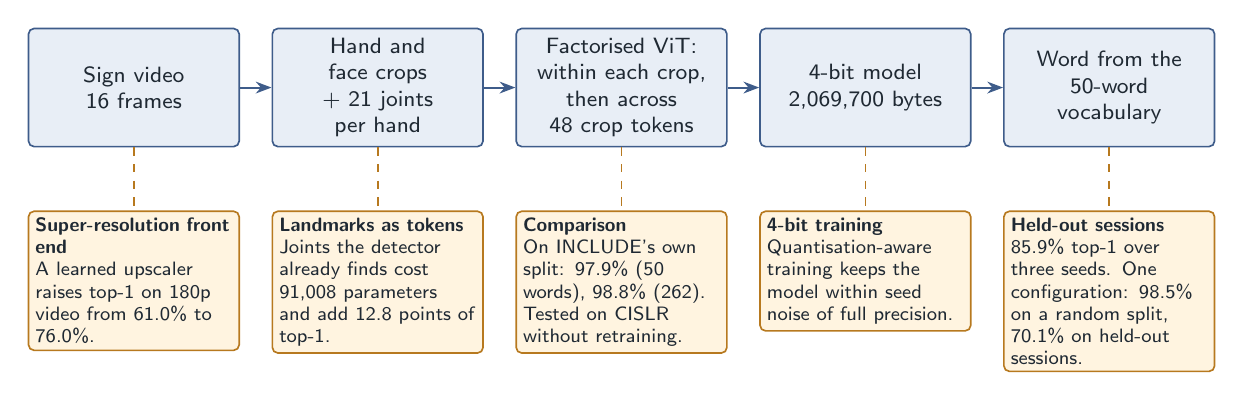
\begin{tikzpicture}[
  font=\sffamily\footnotesize, text=ink,
  st/.style={draw=edge, fill=stage, rounded corners=2pt, line width=0.6pt, align=center, minimum height=15mm, text width=25mm, inner sep=2.5pt},
  co/.style={draw=cedge, fill=contrib, rounded corners=2pt, line width=0.6pt, align=left, text width=25mm, inner sep=2.5pt, font=\sffamily\scriptsize, anchor=north, execute at begin node={\hyphenpenalty=10000\exhyphenpenalty=0}},
  arr/.style={-{Stealth[length=2mm]}, draw=edge, line width=0.7pt},
  link/.style={draw=cedge, line width=0.6pt, dashed},
  node distance=4mm]
\node[st] (in) {Sign video\\16 frames};
\node[st, right=of in] (crop) {Hand and face crops\\+ 21 joints\\per hand};
\node[st, right=of crop] (vit) {Factorised ViT:\\within each crop,\\then across\\48 crop tokens};
\node[st, right=of vit] (q) {4-bit model\\2,069,700 bytes};
\node[st, right=of q] (out) {Word from the\\50-word\\vocabulary};
\draw[arr] (in) -- (crop);
\draw[arr] (crop) -- (vit);
\draw[arr] (vit) -- (q);
\draw[arr] (q) -- (out);
\coordinate (row) at ($(in.south)+(0,-8mm)$);
\node[co] (c4) at (row -| in) {\textbf{Super-resolution front end}\\A learned upscaler raises top-1 on 180p video from 61.0\% to 76.0\%.};
\node[co] (c1) at (row -| crop) {\textbf{Landmarks as tokens}\\Joints the detector already finds cost 91,008 parameters and add 12.8 points of top-1.};
\node[co] (c5) at (row -| vit) {\textbf{Comparison}\\On INCLUDE's own split: 97.9\% (50 words), 98.8\% (262). Tested on CISLR without retraining.};
\node[co] (c2) at (row -| q) {\textbf{4-bit training}\\Quantisation-aware training keeps the model within seed noise of full precision.};
\node[co] (c3) at (row -| out) {\textbf{Held-out sessions}\\85.9\% top-1 over three seeds. One configuration: 98.5\% on a random split, 70.1\% on held-out sessions.};
\foreach \s/\c in {in/c4, crop/c1, vit/c5, q/c2, out/c3} \draw[link] (\s.south) -- (\c.north);
\end{tikzpicture}
\caption{Overview of the proposed work. Blue boxes are the recognition pipeline; each orange box is a contribution, placed under the stage it concerns.}\label{fig:overview}
\end{figure}

The network reads three detected crops per frame (left hand, right hand, face) and adds the 21 hand-joint coordinates of each hand to the hand tokens, so pose information enters the same token stream without a separate pose network. Quantisation-aware training then lets the complete model be stored at 4 bits. On 472 test clips from held-out recording sessions of the INCLUDE corpus, the released model reaches 85.9\% mean top-1 accuracy on 50 words over three seeds.

The evaluation follows how INCLUDE was recorded. When clips from one recording session fall on both sides of the train--test boundary, accuracy can be overstated: on this corpus the same pixel-only configuration scores 98.5\% on a random-video split and 70.1\% on held-out sessions. Trained on INCLUDE's own split, the model scores 97.9\% on 50 words and 98.8\% on 262 words, against previously reported results of 94.5\% and 85.6--97.8\%. The manuscript also scores the released model on CISLR, recorded by other signers with other cameras, and separates the gain of a learned upscaler on low-resolution video from the further gain added by its adversarial loss.

\textbf{Why \textit{Scientific Reports}}

\textit{Scientific Reports} has published several works close to ours in application, and the manuscript compares its results with each of them:
\begin{itemize}\setlength{\itemsep}{1pt}\setlength{\parskip}{0pt}
\item Lamaakal \textit{et al.}, an explainable hybrid CNN--transformer model for sign language recognition on edge devices (\textit{Sci. Rep.} \textbf{16}, 7143; 2026);
\item Venkatappa \textit{et al.}, dynamic Kannada Sign Language recognition on resource-constrained devices (\textit{Sci. Rep.} \textbf{16}, 11186; 2026);
\item Nedungadi \textit{et al.}, a Vision Transformer-powered conversational agent for ISL e-governance accessibility (\textit{Sci. Rep.} \textbf{15}, 33055; 2025).
\end{itemize}
Our work continues this line for Indian Sign Language: it brings a Vision Transformer to the storage budget of an edge device and reports accuracy on recording sessions held out from training. Readers who follow these papers are likely to be the ones who use or test it.

The journal's broad readership is a second reason. The finding that a random split overstates accuracy on a corpus recorded in sessions is relevant to anyone who trains on video recorded in sessions, not only sign language researchers. Finally, the journal judges submissions on scientific validity, and the manuscript is built to be checked: all code, configurations, split definitions, result files and the three released models are in a public repository (\url{https://github.com/not-good-keeper/compact-vit-sign-language}). Open access means that researchers and developers working on assistive technology for the Deaf community in India can read the paper and reuse the models without a subscription.

\textbf{Declarations}

The manuscript is original, has not been published, and is not under consideration at another journal. All authors have read and approved the submission. The authors declare no competing interests. We have had no prior discussions with a \textit{Scientific Reports} Editorial Board Member about this work. We do not suggest reviewers and do not request that any be excluded. A Supplementary Information file accompanies the manuscript.

\textbf{Corresponding author}\\
Bagyammal Thirumurthy\\
Department of Computer Science and Engineering, Amrita School of Computing\\
Amrita Vishwa Vidyapeetham, Coimbatore, India\\
Email: \href{mailto:t_bagyammal@cb.amrita.edu}{t\_bagyammal@cb.amrita.edu}

Thank you for considering this manuscript.

Yours sincerely,

Bagyammal Thirumurthy\\
on behalf of all authors: Nethi Kushala Kumar, Yalamanchi Kushal, Bagyammal Thirumurthy and Dhrusheek Rishi Menon

\end{document}
